\section{Taylor expansion}
So let's first start with a refresher of the Taylor expansion in one dimension.
As you might recall, a Taylor expansion is a way to represent a function as a polynomial. We use this because dealing with polynomials is oftentimes easier than working with the original function.

\subsection{1D-Taylor expansion} 
Generally when we use Taylor-expansion we are not interested in the whole function we are expanding, but only in a small area around a a point $x_0$. The distance between this point and any other close point to it we denote by $\delta x$. We can then express $x$ as follows:
\begin{align}
		x = x_0 + \delta x
\end{align}
From which follows that 
\begin{align} \label{eq:increment}
		\delta x = x - x_0
\end{align}

\begin{figure}[htbp]
	\centering
	% Hier lädst du das fertige PDF, das aus TikZ entstanden ist
	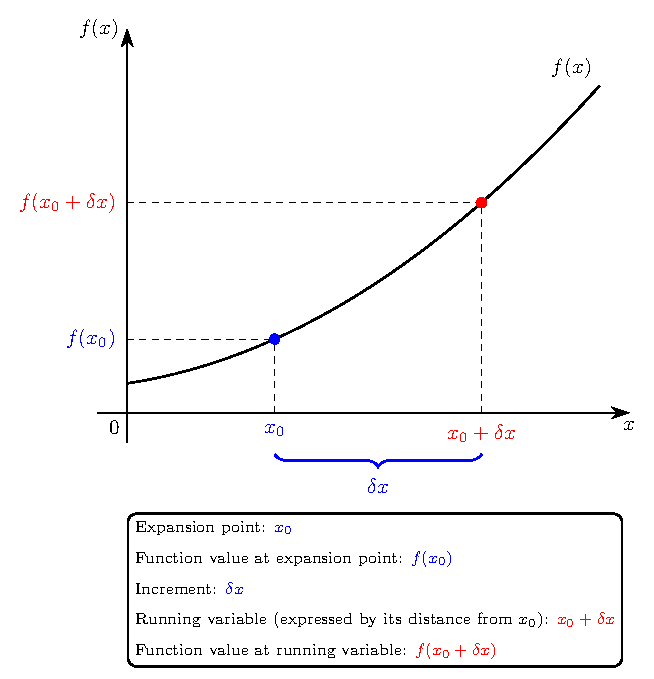
\includegraphics[width=0.8\textwidth]{images/tikz/taylor.pdf}
	\caption{Illustration of the variables for the Taylor expansion.}
	\label{fig:taylor_skizze}
\end{figure}

The formula for the one-dimensional Taylor expansion is given by: 
\begin{align}
    f(x)=f(x_0+\delta x)= \sum_{n=0}^\infty \frac{f^{(n)}(x_0)}{n!}(x-x_0)^n
\end{align}
Where I used the following conventions:
\begin{align}
    f^{(n)}(x_0) = \left[\frac{\text{d}^n}{\text{d}x^n} f(x)\right]\bigg{|}_{x_0}
\end{align}
So $f^{(n)}(x_0)$ means that we derive first and then plug in $x_0$ into that derivative.
Alternatively we can write the Taylor expansion in terms of $\delta x$, using equation (\ref{eq:increment})
\begin{align}\label{eq:taylor1d_increment}
    f(x)=f(x_0+\delta x)= \sum_{n=0}^\infty \frac{f^{(n)}(x_0)}{n!}\delta x^n
\end{align}
$x_0$ is the point that we are developing our Taylor expansion around. 
Let's just do a short example to see how this works and how we can use it to simplify an expression for us. 

\begin{examplebox}{1D-Taylor-Expansion}
	\label{ex:1d-taylor}
	One of the best examples for the use of Taylor expansions is the sine function. 
	Say we observe an oscillation that is in the form of a sine and our goal is to create a somewhat easier representation of the sine expression. We can use a Taylor expansion of the sine function to transform the sine into a polynomial. 
	\tcblower 
	\textbf{Develop sin(x) around $x_0 = 0$} up to the third order¸\\
	The cleanest way to do this is to use expression ($\ref{eq:taylor1d_increment}$). To do this, we first need to calculate $\delta x$
	\begin{align*}
		\delta x = x - x_0 = x 
	\end{align*}
	Easy enough! In the next step we should calculate all the necessary derivatives (or just do it in your head) and evaluate them at $x_0$.
	\begin{align}
		\eval{\dv[0]{}{x}\sin(x)}_{x_0} &= \eval{\sin(x)}_0 = 0 \\
		\eval{\dv[1]{}{x}\sin(x)}_{x_0} &= \eval{\cos(x)}_0 = 1\\
		\eval{\dv[2]{}{x}\sin(x)}_{x_0} &= \eval{-\sin(x)}_0 = 0\\
		\eval{\dv[3]{}{x}\sin(x)}_{x_0} &= \eval{-\cos(x)}_0 = -1\\
	\end{align}
	
	With all this preparation we can start by plugging into our formula:
	\begin{align*}
		f(x)&=f(x_0+\delta x)= \sum_{n=0}^\infty \frac{f^{(n)}(x_0)}{n!}\delta x^n\\
		&= \frac{1}{0!}f^{(0)}(x_0)\delta x^0 + \frac{1}{1!} f^{(1)}(x_0)\delta x^1 +  \frac{1}{2!}f^{(2)}(x_0)\delta x^2 + \frac{1}{3!} f^{(3)}(x_0)\delta x^3 + ...\\
		&= 0 + x + 0 - \frac{1}{6} x^3 +... = x- \frac{1}{6} x^3 +..
	\end{align*}
	Okay, so far this looks a lot easier to use than the abstract sine object. But you might say, okay, how does this help us? We have to calculate an infinite amount of terms! Well, mathematically you are correct. But as physicists, we can apply a little trick. We only consider the number of terms necessary to describe our problem at hand accurately for our needs. Note that in principle we could calculate the result infinitely precise, just by considering more terms in our Taylor expansion. But oftentimes it is sufficient for physicists to consider only the first few terms of this expansion. Let's apply this to our example. Say we are looking at something that oscillates only a tiny amount around $x_0$. So our $\delta x = x-x_0$ term becomes very small. As we chose our $x_0=0$ and (therefore $\delta x = x$), we can just say that $x$ is small in our formula, $x \ll 1$. Therefore, terms of higher order become very small, as they contain higher orders of a very small number. So we might decide that only terms of order three contribute meaningfully to our solution and ignore everything beyond. 
	Our new expression for our sine function now becomes:
	\begin{align}
		\sin(x) \approx x- \frac{1}{6} x^3
	\end{align}
	So we went from a function that we could not really work with to a much simpler representation. This is the power of Taylor expansion and the whole point why we use it. 
	Now let's go to more than one dimension.
\end{examplebox}
\subsection{A more general definition of Taylor expansion}
There is a more general way to express the Taylor expansion. This is useful if you do not want to memorize equation (\ref{eq:taylor1d}) (altough I recommend that for 1D) and more importantely it will simplify the multivariate Taylor expansion which will be covered later. We found that 

\begin{align*}
	f(x)&=f(x_0+\delta x)= \sum_{n=0}^\infty \frac{f^{(n)}(x_0)}{n!}\delta x^n\\
		&= \frac{1}{0!}f^{(0)}(x_0)\delta x^0 + \frac{1}{1!} f^{(1)}(x_0)\delta x^1 +  \frac{1}{2!}f^{(2)}(x_0)\delta x^2 + \frac{1}{3!} f^{(3)}(x_0)\delta x^3 + ...\\
	&= \frac{1}{0!}\delta x^0 \dv[0]{f(x_0)}{x} + \frac{1}{1!} \delta x^1\dv[1]{f(x_0)}{x} +  \frac{1}{2!}\delta x^2\dv[2]{f(x_0)}{x} + \frac{1}{3!} \delta x^3\dv[3]{f(x_0)}{x} + ...\\
\end{align*}
In the last step, I just pulled $\delta x^n$ to the front, the reason for this will become clear in a second. If we take a look at this result it looks oddly similiar to the shape of the series expansion of $e^u$:
\begin{align}
	e^u = 1+u+\frac{u^2}{2}+\frac{u^3}{6}+... = \sum_{n=0}^{\infty} \frac{u^n}{n!}
\end{align}
Actually, if we make the identification
\begin{align*}
	u = \delta x \dv{}{x}
\end{align*}

We can express the Taylor polynomial as 

\begin{align}
f(x)&= \sum_{n=0}^\infty \frac{f^{(n)}(x_0)}{n!}\delta x^n = e^{\delta x \dv{}{x}}f(x_0)\\
\end{align}

Which looks a lot more handy. For one dimension this definition might not be life-changing and I would recommend using the definition we discussed earlier for Problems in 1D, as you save time because you do not have to expand out the exponential function first. However this definition will become extremely useful when we look at the case of multivariate Taylor expansion. 

\subsection{Multivariate Taylor Expansion}
If we want to find a simpler representation for a multivariate function, we must consider the multivariate Taylor Expansion. 
The multivariate Taylor expansion for a function $f(\vec{x})=f(x_1,x_2, \dots, x_n)$ is defined as:
\begin{align}
    T(\vec{x};\vec{a}) = \sum^\infty_{|\vec{\alpha}|=0}\frac{D^{\Vec{\alpha}}f(\vec{x}_0)}{\vec{\alpha}!}\left(\vec{x}-\vec{x_0}\right)^{\vec{\alpha}}
\end{align}
Now this looks very confusing and intimidating if you see it for the first time, but we will dissect it and make sure we understand every part of it, and then do a small example together. Probably the most confusing thing about this definition is the notation. 

\subsubsection*{The Multi-index $\vec{\alpha}$}

The heart of this notation is the vector $\vec{\alpha}$, which is called a Multi-index. 
It acts really just as an index for our sum and is a vector of non-negative whole numbers:
\begin{align}
    \vec{\alpha} = (\alpha_1, \alpha_2, \dots,\alpha_n)
\end{align}
for example:
\begin{align}
    \vec{\alpha} = (2,0,1)
\end{align}
These numbers tell us how often something is supposed to happen with our function. This will become more clear when we look at the example later on. 

\subsubsection*{The dimension of $\vec{\alpha}$}
The dimension $n$ of $\vec{\alpha}$ is the dimension of the variable $\vec{x}$ of the function we are developing.
\begin{align}
    \dim(\vec{\alpha}) = \dim(\vec{x})
\end{align}
So if $\vec{x}$ has three components, our vector $\vec{\alpha}$ also has three components!
Now we need to discuss a very important property of $\vec{\alpha}$ to understand our notation. 

\subsubsection*{The absolute value of $\vec{\alpha}$}
The definition of the absolute value of $\vec{\alpha}$ is not the standard definition for the length of a vector. Instead, it is defined as:
\begin{align}
    |\vec{\alpha}| = \sum_{i=1}^n \alpha_i = \alpha_1+\alpha_2+\dots+\alpha_n
\end{align}
For example:
\begin{align}
    |\vec{\alpha}|=|(2,0,1)| = 2+0+1 = 3
\end{align}

\subsubsection*{The Factorial of $\vec{\alpha}$}
The factorial of our Multi-index $\vec{\alpha}$ is defined as:
\begin{align}
    \vec{\alpha}! = \alpha_1!\cdot\alpha_2!\,\cdot\dots\cdot\,\alpha_n! = \prod_{i=1}^n \alpha_i!
\end{align}

\subsubsection*{The Derivative $D^{\vec{\alpha}}$}
This derivative term might seem like the most difficult of our definitions, but is actually very easy to understand. It is defined as:
\begin{align}
    D^{\vec{\alpha}}=\frac{\partial^{|\vec{\alpha}|}}{\partial x_1^{\alpha_1}\cdot \partial x_2^{\alpha_2}\cdot\partial x_3^{\alpha_3}\cdot\dots\cdot\partial x_n^{\alpha_n}}
\end{align}
For our example, this would be:
\begin{align}
    D^{(2,0,1)}=\frac{\partial^3}{\partial x_1^2 \cdot \partial x_2^0 \cdot \partial x_3^1}
\end{align}
Okay, now that we have got all these definitions, we want to think a little bit about what is happening in our Multivariate Taylor Expansion.
Essentially, if we look back at our formula, this is what it tells us:
We go through all possible combinations of our Multi-index $\alpha$ that have a certain absolute value, associated with the current summation term. 
Note that $D^{\vec{\alpha}}f(\vec{x}_0)$ just like in one dimension denotes that we \textit{first} apply the derivative and \textit{then} plug in our point of development $x_0$.

\subsubsection*{1st Step: $|\vec{\alpha}|=0$}
For example, let's say our $|\vec{\alpha}|=0$. That means we only have one combination of indices that can make that happen, and that is:
\begin{align}
    \vec{\alpha}=(0,0,0)
\end{align}
So now all we have to do is to use our definitions from above and plug in all these values to obtain the first term of our expansion. 

\subsubsection*{2nd Step: $|\vec{\alpha}|=1$}
Now if $|\vec{\alpha}|=1$, the situation becomes a bit more complex, because we have three possible arrangements of $\vec{\alpha}$ that produce this absolute value:
\begin{align}
    \vec{\alpha} &= (1,0,0) \\
    \vec{\alpha} &= (0,1,0) \\
    \vec{\alpha} &= (0,0,1)
\end{align}
To get our next terms of summation, we have to plug in all these three combinations into our definitions and add the result.

\subsubsection*{3rd Step: $|\vec{\alpha}|=2$}
By continuing this process, you can then find for our next step $|\vec{\alpha}|=2$: 
\begin{align}
    \vec{\alpha} &= (1,1,0) \\
    \vec{\alpha} &= (0,1,1) \\
    \vec{\alpha} &= (1,0,1) \\
    \vec{\alpha} &= (2,0,0) \\
    \vec{\alpha} &= (0,2,0) \\
    \vec{\alpha} &= (0,0,2)
\end{align}
Again, we have to plug in all of these into our definitions to obtain all the terms that we need in this step. 
This process continues then into infinity.

\subsubsection*{The Bracket raised to the power of a Vector}
There is one last aspect of multivariate Taylor expansion that we should talk about. The meaning of:
\begin{align}\label{eq:differencetaylor}
    (\vec{x}-\vec{x}_0)^{\vec{\alpha}}
\end{align}
To explain this, I have to explicitly write out $\vec{x}_0$:
\begin{align}
    \vec{x}_0=(x_{01}, x_{02})
\end{align}
Expression (\ref{eq:differencetaylor}) seems extremely confusing at first because what does it mean to raise a vector by another vector? Well, in our convention, there is a clear definition of this, and it's really simple:
\begin{align}
    (\vec{x}-\vec{x}_0)^{\vec{\alpha}} = \left((x_1-x_{01}), (x_2-x_{02})\right)^{(\alpha_1, \alpha_2)} = (x_1-x_{01})^{\alpha_1}\cdot(x_2-x_{02})^{\alpha_2}
\end{align}
We are multiplying all our components, raised to the power of the corresponding component of $\vec{\alpha}$.

\subsubsection*{Example of Multivariate Taylor Expansion}
After this long theoretical preparation, let's do a simple example to illustrate the process in practice.
Let's take a look at the function:
\begin{align}
f(x_1,x_2) = e^{x_1} \cos(x_2)    
\end{align}
Now we want to find a simpler expression for this. For this purpose, we can use our trusted tool, the Taylor Expansion, to find a simpler polynomial representation for this function. As you can see, the function depends on two variables, $x_1$ and $x_2$. Therefore, we have to use the Multivariate Taylor Expansion in this case.

\subsubsection*{Preparations}
Before we start with the expansion, we have to do some preparations. We have to choose a point of development $\vec{x}_0$. Normally, as physicists, we want to choose this point exactly at the position we are interested in, because only then later can we argue that we can throw away terms and still have an accurate description of the problem. In practice, you can often choose your coordinate system so that $\vec{x}_0$ becomes $\vec{0}$, which then simplifies the calculations. So we are going to choose $\vec{x}_0=\vec{0}$ in this example for convenience.
\begin{align}
    \vec{x}_0= \vec{0}
\end{align}
Our $\vec{x}$ is of course:
\begin{align}
    \vec{x}=(x_1, x_2)
\end{align}

\subsubsection*{1st Step ($|\vec{\alpha}|=0$)}

\begin{table}[h!]
    \centering
    \renewcommand{\arraystretch}{1.5} 
    \begin{tabular}{cccc}
        \hline
        $|\vec{\alpha}|=0$ & $D^{\vec{\alpha}}$ & $\left(\vec{x}-\vec{x_0}\right)^{\vec{\alpha}}$& $\vec{\alpha}!$\\
        \hline
        $(\alpha_1, \alpha_2)=(0, 0)$&$\frac{\partial^0}{\partial x_1^{0}\cdot \partial x_2^{0}}$& $(x_1-0)^0\cdot(x_2-0)^0$& $0!\cdot0!= 1$
    \end{tabular}
    \label{tab:taylor_example_1}
\end{table}
Now that we have found these important components, we can proceed and plug in our actual values: 
\begin{align}
        T_{(0,0)}&=\frac{1}{1}\left[\frac{\partial^0}{\partial x_1^{0}\cdot \partial x_2^{0}} f(x_1, x_2)\right]\bigg{|}_{(0,0)}(x_1-0)^0\cdot(x_2-0)^0\\
        &=f(0,0)= e^{0} \cos(0) = 1
\end{align}
This already was our first step! Now let's go to the second step...

\subsubsection*{2nd Step ($|\vec{\alpha}|=1$)}

\begin{table}[h!]
    \centering
    \renewcommand{\arraystretch}{1.5} 
    \begin{tabular}{cccc}
        \hline
        $|\vec{\alpha}|=1$ & $D^{\vec{\alpha}}$ & $\left(\vec{x}-\vec{x_0}\right)^{\vec{\alpha}}$& $\vec{\alpha}!$\\
        \hline
        $(\alpha_1, \alpha_2)=(1, 0)$&$\frac{\partial^1}{\partial x_1^{1}\cdot \partial x_2^{0}}$& $(x_1-0)^1\cdot(x_2-0)^0$ & $1!\cdot 0! = 1$\\
        $(\alpha_1, \alpha_2)=(0, 1)$&$\frac{\partial^1}{\partial x_1^{0}\cdot \partial x_2^{1}}$& $(x_1-0)^0\cdot(x_2-0)^1$ &$0!\cdot 1! = 1$
    \end{tabular}
    \label{tab:taylor_example_2}
\end{table}
Now we again have the important components, and we can proceed to plug in our actual values: 
\begin{align}
        T_{(1,0)}&=\frac{1}{1}\left[\frac{\partial^1}{\partial x_1^{1}\cdot \partial x_2^{0}}f(x_1, x_2)\right]\bigg{|}_{(0,0)}(x_1-0)^1\cdot(x_2-0)^0\\
        &=\eval{\frac{\partial}{\partial x_1}f(x_1,x_2)}_{(0,0)}x_1= \eval{\left[e^{x_1} \cos(x_2)\right]}_{(0,0)}x_1= x_1
\end{align}
Now we have to repeat this step for $T_{(0,1)}$:
\begin{align}
        T_{(0,1)}&=\frac{1}{1}\left[\frac{\partial^1}{\partial x_1^{0}\cdot \partial x_2^{1}}f(x_1, x_2)\right]\eval_{(0,0)}(x_1-0)^0\cdot(x_2-0)^1\\
        &=\eval{\frac{\partial}{\partial x_2}f(x_1,x_2)}_{(0,0)}x_2= \eval{\left[-e^{x_1} \sin(x_2)\right]}_{(0,0)}= 0
\end{align}

\subsubsection*{3rd Step ($|\vec{\alpha}|=2$)}
Now let's do a third and final step to finalize this example.
\begin{table}[h!]
    \centering
    \renewcommand{\arraystretch}{1.5} 
    \begin{tabular}{cccc}
        \hline
        $|\vec{\alpha}|=2$ & $D^{\vec{\alpha}}$ & $\left(\vec{x}-\vec{x_0}\right)^{\vec{\alpha}}$& $\vec{\alpha}!$\\
        \hline
        $(\alpha_1, \alpha_2)=(1, 1)$&$\frac{\partial^2}{\partial x_1^{1}\cdot \partial x_2^{1}}$& $(x_1-0)^1\cdot(x_2-0)^1$ &$1!\cdot 1! = 1$\\
        $(\alpha_1, \alpha_2)=(2, 0)$&$\frac{\partial^2}{\partial x_1^{2}\cdot \partial x_2^{0}}$& $(x_1-0)^2\cdot(x_2-0)^0$ &$2!\cdot 0! = 2$\\
        $(\alpha_1, \alpha_2)=(0, 2)$&$\frac{\partial^2}{\partial x_1^{0}\cdot \partial x_2^{2}}$& $(x_1-0)^0\cdot(x_2-0)^2$ &$0!\cdot 2! = 2$
    \end{tabular}
    \label{tab:taylor_example_3}
\end{table}
\begin{align}
        T_{(1,1)}&=\frac{1}{1}\left[\frac{\partial^2}{\partial x_1^{1}\cdot \partial x_2^{1}}f(x_1, x_2)\right]\eval_{(0,0)}(x_1-0)^1\cdot(x_2-0)^1\\
        &=\eval{\frac{\partial}{\partial x_1}\frac{\partial}{\partial x_2}f(x_1,x_2)}_{(0,0)}x_1\, \cdot x_2=  \eval{\left[-e^{x_1}\sin(x_2)\right]}_{(0,0)}= 0
\end{align}
\begin{align}
T_{(2,0)}&=\frac{1}{2}\left[\frac{\partial^2}{\partial x_1^{2}\cdot \partial x_2^{0}}f(x_1, x_2)\right]\eval_{(0,0)}(x_1-0)^2\cdot(x_2-0)^0\\
&=\frac{1}{2}\eval{\frac{\partial^2}{\partial x_1^2}f(x_1,x_2)}_{(0,0)}x_1^2 =  \frac{1}{2}\eval{\left[e^{x_1}\cos(x_2)\right]}_{(0,0)}x_1^2=\frac{1}{2}x_1^2
\end{align}
\begin{align}
T_{(0,2)}&=\frac{1}{2}\left[\frac{\partial^2}{\partial x_1^{0}\cdot \partial x_2^{2}}f(x_1, x_2)\right]\eval_{(0,0)}(x_1-0)^0\cdot(x_2-0)^2\\
&=\frac{1}{2}\eval{\frac{\partial^2}{\partial x_2^2}f(x_1,x_2)}_{(0,0)}x_2^2 = \frac{1}{2} \eval{\left[-e^{x_1}\cos(x_2)\right]}_{(0,0)}x_2^2=-\frac{1}{2}x_2^2
\end{align}
\subsection*{Putting it all together}
Okay, now that we have found all of those terms, let's put them together:
\begin{align}
    f(x_1, x_2)=e^{x_1} \cos(x_2)  \approx 1+ x_1+ \frac{x_1^2}{2}-\frac{x_2^2}{2} 
\end{align}

\subsection{A Practical Method for Taylor-Expansion}

Now that we understood the basics of Taylor-Expansion we can move on to a more
advanced but very useful method of conducting the Taylor-Expansion and we will
use it a lot later on. We will encounter Taylor Expansions of functions that look for example like this
\begin{align}
	f(x+\epsilon)
\end{align}
You can do this of course with the methods we discussed earlier, but there is a simple way to do it and you will never struggle with any Taylor Expansion again.

\subsubsection*{One Dimension}

Let us go back to one dimension first.  Imagine you have a function $f$ and it depends on some argument. This argument could be anything and we are free to choose the shape of the argument so that it suits our needs as physicists. Lets look an example to illustrate this.
We can define a function $f(x)$ as
\begin{align}
	f(x) = x^2
\end{align}
If we plug in $3$ now, we get $f(3)=9$ as a result.
But maybe we are in a situation where we want to simplify the function for some reason. Then we could also write it as follows:
\begin{align}
	f(x^2)=x
\end{align}
If we plug in $3$ again now, we obtain the same result, but somewhat simplified our expression. 
The function $f(x)$ acts like a machine with a slot. This gives us the freedom to choose our slot just as we need it to and we call this slot $u$. So when we encounter a function $f(x)$ we can cleverly choose our $u$ and rewrite $f(x)\rightarrow f(u)$.
In our example then we would get the following, if we chose $u=x^2$
\begin{align}
	f(u)=u\,.
\end{align}

Now we want to move on to how to Taylor-Expand this function.

 

\noindent This leads to the following five-step recipe.

\paragraph{Recipe (1D).}
\begin{enumerate}
	\item \textbf{Name the argument.}
	Identify what stands inside the parentheses of $f(\,\cdot\,)$ and
	call it $u$.  Then $f$ is a function of $u$ alone: $f = f(u)$.
	
	\item \textbf{Determine the expansion point.}
	Evaluate $u$ at the expansion point $x_0$:
	\begin{equation}
		u_0 \;=\; u(x_0).
	\end{equation}
	This gives a concrete number (or symbol) around which we expand.
	
	\item \textbf{Compute the perturbation.}
	Find how much $u$ changes when $x$ is shifted away from $x_0$:
	\begin{equation}
		\delta u \;=\; u(x_0 + \varepsilon) - u(x_0).
	\end{equation}
	Note carefully: we substitute $x_0$, \emph{not} a free variable $x$,
	into the argument.
	
	\item \textbf{Compute the derivative.}
	Differentiate $f$ with respect to its argument $u$ and evaluate at
	$u_0$:
	\begin{equation}
		f'(u_0) \;=\; \left.\frac{\mathrm{d}f}{\mathrm{d}u}\right|_{u\,=\,u_0}.
	\end{equation}
	
	\item \textbf{Insert into the Taylor formula.}
	To first order in $\varepsilon$:
	\begin{equation}
		\boxed{f\bigl(u_0 + \delta u\bigr)
			\;\approx\; f(u_0) \;+\; f'(u_0)\cdot\delta u.}
		\label{eq:taylor1d}
	\end{equation}
	Higher-order corrections are obtained by including the terms
	$\tfrac{1}{n!}f^{(n)}(u_0)\,(\delta u)^n$ for $n \geq 2$.
\end{enumerate}

\paragraph{Example: the free-particle Lagrangian.}
The Lagrangian of a free particle depends only on the squared speed
$L = L(v^2)$.  Under a Galilean boost by a small velocity $\varepsilon$ the
speed changes as $v \mapsto v' = v + \varepsilon$, so the argument of $L$
becomes $(v+\varepsilon)^2$.

\begin{enumerate}
	\item \textbf{Argument:} $u = v^2$, so $L = L(u)$.
	\item \textbf{Expansion point:} $u_0 = v^2$ (a symbol, since we do not
	fix $v$).
	\item \textbf{Perturbation:}
	\begin{equation}
		\delta u
		= u(v+\varepsilon) - u(v)
		= (v+\varepsilon)^2 - v^2
		= 2v\varepsilon + \varepsilon^2.
	\end{equation}
	\item \textbf{Derivative:} $\displaystyle\frac{\partial L}{\partial(v^2)}$,
	evaluated at $u_0 = v^2$.
	\item \textbf{Result (to first order in $\varepsilon$):}
	\begin{equation}
		L' \;\approx\; L(v^2) \;+\; \frac{\partial L}{\partial(v^2)}
		\cdot 2v\varepsilon.
	\end{equation}
\end{enumerate}

\noindent Galilean invariance then requires the extra term to be a total time
derivative for all trajectories, which forces
$\partial L/\partial(v^2) = \mathrm{const}$ and hence $L \propto v^2$.

%-----------------------------------------------------------------------
\subsubsection*{Multiple Dimensions}
%-----------------------------------------------------------------------

The recipe generalises immediately to functions of several variables.  Let
$f$ depend on arguments $u_1, u_2, \ldots, u_d$, each of which is a function
of $\boldsymbol{x} = (x_1, \ldots, x_n)$.  We expand around a point
$\boldsymbol{x}_0$.

\paragraph{Recipe (multi-dimensional).}

Steps 1--3 are carried out for \emph{each} argument independently:
\begin{align}
	u_{i,0} &= u_i(\boldsymbol{x}_0), \\
	\delta u_i &= u_i(\boldsymbol{x}_0 + \boldsymbol{\varepsilon})
	- u_i(\boldsymbol{x}_0).
\end{align}
Step 4 now yields one \emph{partial} derivative per argument.  The first-order
result is the sum of all individual corrections:
\begin{equation}
	\boxed{f(u_{1,0}+\delta u_1,\ldots) \;\approx\; f(u_{1,0},\ldots)
		\;+\; \sum_{i}\,\frac{\partial f}{\partial u_i}\bigg|_{\boldsymbol{u}_0}
		\cdot\,\delta u_i.}
	\label{eq:taylor_md_1}
\end{equation}

To go to \textbf{second order} one must also include all mixed second
derivatives.  Using the multi-index notation
$\alpha = (\alpha_1,\ldots,\alpha_d)$ with
$|\alpha|=\alpha_1+\cdots+\alpha_d$ and
$\alpha! = \alpha_1!\cdots\alpha_d!$, the full expansion reads:
\begin{equation}
	f(\boldsymbol{u}_0 + \delta\boldsymbol{u})
	\;=\; \sum_{|\alpha|\leq N}
	\frac{1}{\alpha!}\,\bigl(\partial^{\alpha}f\bigr)(\boldsymbol{u}_0)
	\,(\delta\boldsymbol{u})^{\alpha}
	\;+\; \mathcal{O}\!\left(|\delta\boldsymbol{u}|^{N+1}\right),
	\label{eq:taylor_multiindex}
\end{equation}
where $\partial^{\alpha}f = \partial^{|\alpha|}f /
(\partial u_1^{\alpha_1}\cdots\partial u_d^{\alpha_d})$ and
$(\delta\boldsymbol{u})^{\alpha}=\prod_i(\delta u_i)^{\alpha_i}$.

In two dimensions with $u$ and $v$, the terms up to second order are:
\begin{equation}
	f \;\approx\; f_0
	\;+\; \frac{\partial f}{\partial u}\,\delta u
	\;+\; \frac{\partial f}{\partial v}\,\delta v
	\;+\; \frac{1}{2}\frac{\partial^2 f}{\partial u^2}\,(\delta u)^2
	\;+\; \frac{\partial^2 f}{\partial u\,\partial v}\,\delta u\,\delta v
	\;+\; \frac{1}{2}\frac{\partial^2 f}{\partial v^2}\,(\delta v)^2,
	\label{eq:taylor2d}
\end{equation}
where all derivatives are evaluated at $(u_0,v_0)$.  The mixed term
$\partial^2 f/\partial u\,\partial v$ appears with coefficient $1$ (not
$\tfrac{1}{2}$) because by Schwarz's theorem
$\partial_{uv}f = \partial_{vu}f$, and both orderings contribute.

\paragraph{Example: $f(x,y)=e^x\cos y$ around $(0,0)$.}

\begin{enumerate}
	\item \textbf{Arguments:} $u=x$, $v=y$; expansion point $u_0=v_0=0$;
	$f(0,0)=1$.
	\item \textbf{Perturbations:} $\delta u = x$, $\delta v = y$.
	\item \textbf{Partial derivatives at $(0,0)$:}
	\begin{align*}
		\partial_x f &= e^x\cos y \;\to\; 1, &
		\partial_y f &= -e^x\sin y \;\to\; 0,\\
		\partial_{xx}f &= e^x\cos y \;\to\; 1, &
		\partial_{yy}f &= -e^x\cos y \;\to\; -1, &
		\partial_{xy}f &= -e^x\sin y \;\to\; 0.
	\end{align*}
	\item \textbf{Result (to second order):}
	\begin{equation}
		e^x\cos y \;\approx\; 1 \;+\; x \;+\; \tfrac{1}{2}x^2
		\;-\; \tfrac{1}{2}y^2.
	\end{equation}
\end{enumerate}

\noindent As a consistency check, setting $y=0$ recovers $e^x\approx
1+x+\tfrac{1}{2}x^2$, and setting $x=0$ recovers $\cos y\approx
1-\tfrac{1}{2}y^2$, both of which are the familiar one-dimensional results.
